%%%%%%%%%%%%%%%%%%%%%%%%%%%%%%%%% LAB-5 %%%%%%%%%%%%%%%%%%%%%%%%%%%%%%%%%%
%>>>>>>>>>>>>>>>>>>>>>>>>>> ПЕРЕМЕННЫЕ >>>>>>>>>>>>>>>>>>>>>>>>>>>>>>>>>>>
%>>>>> Информация о кафедре
%\newcommand{\year}{2021 г.}  % Год устанавливается автоматически
\newcommand{\city}{Санкт-Петербург}  %  Футер, нижний колонтитул на титульном листе
\newcommand{\university}{Национальный исследовательский университет ИТМО}  % первая строка
\newcommand{\department}{Факультет программной инженерии и компьютерной техники}  % Вторая строка
\newcommand{\major}{Направление программная инженерия}  % Треьтя строка
% Пусть будет. Проще закоментить лишнее.
\newcommand{\education}{Образовательная программа системное и прикладное программное обеспечение}  % четвертая строка
\newcommand{\specialization}{Специализация системное программное обеспечение}  % пятая строка

%<<<<< Информация о кафедре

%>>>>> Назание работы
\newcommand{\reporttype}{ОТЧЕТ ПО ДОМАШНЕЙ РАБОТЕ} % тип работы, (главный заголовок титульного листа)
\newcommand{\lab}{Лабораторная работа}          % вид работы
\newcommand{\labnumber}{№ 2}                    % порядковый номер работы
\newcommand{\subject}{Компьютерные сети}         % учебный предмет
\newcommand{\labtheme}{Моделирование компьютерных сетей в среде NetEmul: Локальные сети}            % Тема лабораторной работы

\newcommand{\student}{Тюрин Иван Николаевич}    % определение ФИО студента
\newcommand{\studygroup}{P33102}                 % определение учебной группы 
\newcommand{\teacher}{% принимающий
    Авксентьева Е. Ю.,\\[1mm]% ФИО лектора
     Алиев Т. И.% ФИО практика
}

%>>>>>>>>>>>>>>>>>>>>>> ПРЕАМБУЛА >>>>>>>>>>>>>>>>>>>>>>>>>

%>>>>>>>>>>>>>>>>>> ПРЕАМБУЛА >>>>>>>>>>>>>>>>>>>>
\documentclass[14pt,final,oneside]{extreport}% класс документа, характеристики
%>>>>> Разметка документа
\usepackage[a4paper, mag=1000, left=3cm, right=1.5cm, top=2cm, bottom=2cm, headsep=0.7cm, footskip=1cm]{geometry} % По ГОСТу: left>=3cm, right=1cm, top=2cm, bottom=2cm,
\linespread{1} % межстройчный интервал по ГОСТу := 1.5
%<<<<< Разметка документа

%>>>>> babel c языковым пакетом НЕ должны быть первым импортируемым пакетом
\usepackage[utf8]{inputenc}
\usepackage[T1,T2A]{fontenc}
\usepackage[russian]{babel}
%<<<<<

%\usepackage{cmap} %поиск в pdf

%>>>...>> прочие полезные пакеты
\usepackage{amsmath,amsthm,amssymb}
\usepackage{mathtext}
\usepackage{indentfirst}
\usepackage{graphicx}
\usepackage{float}
\graphicspath{{/home/ivan/itmo/informatics/latex}}
\DeclareGraphicsExtensions{.pdf,.png,.jpg}
%\usepackage{bookmark}

\usepackage[dvipsnames]{xcolor}
\usepackage{hyperref}  % Использование ссылок
\hypersetup{%  % Настройка разметки ссылок
    colorlinks=true,
    linkcolor=blue,
    filecolor=magenta,      
    urlcolor=magenta,
    %pdftitle={Overleaf Example},
    %pdfpagemode=FullScreen,
}

\usepackage{diagbox}
\usepackage[letterspace=150]{microtype} % Спэйсинг (межбуквенный интервал для саголовка) \lsstyle
% \usepackage{csvsimple} %импорт содержимого таблицы из csv

%>>> верстка в 2 колонки
\usepackage{multicol} % многоколоночная верстка
\setlength{\columnsep}{.15\textwidth} % определение ширины разделителя между колонками

\usepackage{tikz} % пакет для векторной графики, чтобы рисовать красивый разделитель колонок
% %> кастомный разделитель колонок
% \usetikzlibrary{arrows.meta,decorations.pathmorphing,backgrounds,positioning,fit,petri}
% \usepackage{multicolrule} % Для кастомизации разделителя колонок
% \SetMCRule{                     % кастомизация разделителя колонок multicolrule
%     width=2pt,
%     custom-line={               % Tikz код для кастомизации линии разделителя
%         \draw [                 % Рисовать
%             decorate,           % декорированную (требуются спец настройки пакетов tikz (см. импорт выше)
%             decoration={        % вид декорирования
%                 snake, % Тип - змейка (волнистая)
%                 amplitude=.5mm, % ширина волн
%                 pre length=0mm, % участок прямой линии от начала
%                 %segment length=0mm, % учасок волнистой линии
%                 post length=0mm % участок прямой линии от конца
%             },
%             line width=1pt,
%             step=10pt
%         ] 
%         (TOP) to (BOT); % сверху и до низа колонки
%     }, 
%     extend-top=-5pt, % Вылезти за верхнюю границу колонки 
%     extend-bot=-7pt % Вылезти за нижнюю границу колонки  
% }
%% < кастомный разделитель колонок
%%<<< верстка в 2 колонки

%>>>>> Использование листингов
\usepackage{listings} 
\usepackage{caption}
\DeclareCaptionFont{white}{\color{white}} 
\DeclareCaptionFormat{listing}{\colorbox{gray}{\parbox{\textwidth}{#1#2#3}}}

\captionsetup[lstlisting]{format=listing,labelfont=white,textfont=white} % Настройка вида описаний
\lstset{  % Настройки вида листинга
inputencoding=utf8, extendedchars=\true, keepspaces = true, % поддержка кириллицы и пробелов в комментариях
language={},            % выбор языка для подсветки (здесь это Pascal)
basicstyle=\small\sffamily, % размер и начертание шрифта для подсветки кода
numbers=left,               % где поставить нумерацию строк (слева\справа)
numberstyle=\tiny,          % размер шрифта для номеров строк
stepnumber=1,               % размер шага между двумя номерами строк
numbersep=5pt,              % как далеко отстоят номера строк от подсвечиваемого кода
backgroundcolor=\color{white}, % цвет фона подсветки - используем \usepackage{color}
showspaces=false,           % показывать или нет пробелы специальными отступами
showstringspaces=false,     % показывать илигнет пробелы в строках
showtabs=false,             % показывать или нет табуляцию в строках
frame=single,               % рисовать рамку вокруг кода
tabsize=2,                  % размер табуляции по умолчанию равен 2 пробелам
captionpos=t,               % позиция заголовка вверху [t] или внизу [b] 
breaklines=true,            % автоматически переносить строки (да\нет)
breakatwhitespace=false,    % переносить строки только если есть пробел
escapeinside={\%*}{*)}      % если нужно добавить комментарии в коде
}

\definecolor{codegreen}{rgb}{0,0.6,0}
\definecolor{codegray}{rgb}{0.5,0.5,0.5}
\definecolor{codepurple}{rgb}{0.58,0,0.82}
\definecolor{backcolour}{rgb}{0.95,0.95,0.92}

\lstdefinestyle{mystyle}{
    backgroundcolor=\color{backcolour},   
    commentstyle=\color{codegreen},
    keywordstyle=\color{magenta},
    numberstyle=\tiny\color{codegray},
    stringstyle=\color{codepurple},
    basicstyle=\ttfamily\footnotesize,
    breakatwhitespace=false,         
    breaklines=true,                 
    captionpos=b,                    
    keepspaces=true,                 
    numbers=left,                    
    numbersep=5pt,                  
    showspaces=false,                
    showstringspaces=false,
    showtabs=false,                  
    tabsize=2
}
\lstset{style=mystyle}
%<<<<< Использование листингов


\sloppy % Решение проблем с переносами (с. 119 книга Львовского)
\emergencystretch=25pt


%>>>>>>>>>>>>>>>> ДОПОЛНИТЕЛЬНЫЕ КОМАНДЫ {Для соответствия ГОСТ} >>>>>>>>>>>>>>
%>>>>>> математические функции для удобства
\newcommand{\tx}{\text}
\newcommand{\eps}{\varepsilon}
\renewcommand{\phi}{\varphi}
\newcommand{\limit}{\displaystyle\lim}
\newcommand{\oo}{\infty}
\newcommand{\De}{\Delta}
\newcommand{\cd}{\cdot}
\newcommand{\df}{\partial}
\newcommand{\ndash}{\textendash}
\newcommand{\mdash}{\textemdash}

%>>>>> Аннотирование
\newcommand{\note}[2]{\overbrace{#1}^{#2}}% скобка сверху для комментария
% \overset{}{}% для указания символа над другим смиволом
% \underset{}{}% для указания символа под другим смиволом
%<<<<< Аннотирование

%>>>>>> Матрицы
\DeclareMathOperator{\rank}{rank}
\newcommand{\tvec}[1]{\mathbfit{#1}}% "text vector"
\newcommand{\mtx}[1]{\mathrm{#1}}
\newcommand{\transposed}[1]{{#1}^{\mathrm{T}}}
%>>>>>> Матрицы

%>>>>> Скобки
\newcommand{\lt}{\left}
\newcommand{\rt}{\right}
\newcommand{\la}{\langle}% '<'
\newcommand{\ra}{\rangle}% '>'
\newcommand{\avg}[1]{\langle{#1}\rangle}% '<X>'
%<<<<< Скобки

%>>>>> Дроби
\newcommand{\cf}[2]{\cfrac{#1}{#2}}
\newcommand{\fr}[2]{\frac{#1}{#2}}
%<<<<< Дроби


%>>>>> Стрелки
\newcommand{\Rarr}{\Rightarrow}% ⇒ следствие | лучше использовать \implies
\newcommand{\LRarr}{\Leftrightarrow}% равносильно | лучше  использовать \iff
\newcommand{\rarr}{\xrightarrow{}}% → стрелка вправо
\newcommand{\nwarr}{\nwarrow}% ↖ север-запад стрелка
\newcommand{\nearr}{\nearrow}% ↗ север-восток стрелка
\newcommand{\swarr}{\swarrow}% ↙ юг-запад стрелка
\newcommand{\searr}{\searrow}% ↘ юг-восток стрелка

\newcommand{\raises}{\nwarrow}% возрастает
\newcommand{\increases}{\nwarrow}% возрастает
\newcommand{\falls}{\swarrow}% убывает
\newcommand{\decreases}{\swarrow}% убывает

%{{{
\makeatletter
\newcommand{\impliesby}[2][]{\ext@arrow 0359\Leftrightarrowfill@{#1}{#2}}% следствие с надписью
\makeatother
%}}}

%{{{
\makeatletter
\newcommand{\iffby}[2][]{\ext@arrow 0359\Rightarrowfill@{#1}{#2}}% равносильность с надписью
\makeatother
%}}}
%<<<<< Стрелки

% Функции для удобного описания формул: https://tex.stackexchange.com/questions/95838/how-to-write-a-perfect-equation-parameters-description



%<<<<<< математические функции для удобства
%>>>>>> Стиль текста
\newcommand{\hex}[1]{\texttt{0{\footnotesize{x}}#1}}
\newcommand{\ttt}[1]{\texttt{#1}}
%<<<<<< Стиль текста

\newcommand\Chapter[3]{%
    % Принимает 3 аргумента - название главы и дополнительный заголовок и множитель ширины загловка (можно ничего)
    \refstepcounter{chapter}%
    \chapter*{%
        %\hfill % заполнение отступом пространства до заголовка
        \begin{minipage}{#3\textwidth} % Можно изменить ширину министраницы (заголовка)
            \flushleft % Выранивание заголовка по левому краю параграфа (заголовка)
            %\flushright % Выранивание заголовка по правому краю параграфа (заголовка)
            \begin{huge}%
                % Отключена нумерация глав в тексте:
                % \textbf{\chaptername\ \arabic{chapter}\\}
                \textbf{#1}% Первый заголовок
            \end{huge}%
            \\% Перенос сторки
            \begin{Huge}
                #2% Второй заголовок
            \end{Huge}
        \end{minipage}
    }%
    % Отключена нумерация для chapter в toc (table of contents), т.е. Оглавлении (Содержании):
    % \addcontentsline{toc}{chapter}{\arabic{chapter}. #1}
    % Представление главы в содержании:
    \addcontentsline{toc}{chapter}{#1. #2}%
}

\newcommand\Section[1]{
    % Принимает 1 аргумент - название секции
    \refstepcounter{section}
    \section*{%
        \raggedright
        % Отключена дополнительная нумерация chapter в section в тексте документа:
        % \arabic{chapter}.\arabic{section}. #1}
        % Отключена любая нумарация section в тексте документа: 
        \arabic{section}. #1%
    }
    
    % Отключена дополнительная нумерация chapter в section в toc (table of contents) Оглавлении (Содержании):
    % \addcontentsline{toc}{section}{\arabic{chapter}.\arabic{section}. #1}
    \addcontentsline{toc}{section}{\arabic{section}. #1} 
}


\newcommand\Subsection[1]{
    % Принимает 1 аргумент - название подсекции
    \refstepcounter{subsection}
    \subsection*{%
        \raggedright%
        % Отключена дополнительная нумерация chapter в section в тексте документа (можно добавить отступ с помощью \hspace*{12pt}):
        % \arabic{chapter}.\arabic{section}.\arabic{subsection}. #1}
        \arabic{section}. \arabic{subsection}. #1
    }
    % Отключена дополнительная нумерация chapter в section в Оглавлении (Содержании):
    %\addcontentsline{toc}{subsection}{\arabic{chapter}.\arabic{section}.\arabic{subsection}. #1}
    \addcontentsline{toc}{subsection}{\arabic{subsection}. #1}
}


\newcommand\Figure[4]{
    % Принимает 4 аргумента - название файла изображения, ее размер в тексте, описание, лэйбл (псевдоним в формате "fig:name") 
    %
    \refstepcounter{figure}
    \begin{figure}[H] %- \usepackage {float} %[h]
        \begin{center}
            \fbox{
                \includegraphics[width=#2]{#1}
            }
        \end{center}
        \begin{center}
            Рис.~\arabic{figure}. #3.
        \end{center}
        %\caption{#3}
        \label{fig:#4}
    \end{figure}
}


\newcommand\Table[3]{
    % Принимает 3 аргумента --- лэйбл name(#1) (псевдоним в формате "tab:name"), ее описание(#2), содержание таблицы(#3)
    % ВАЖНО!: от этого способа страдает нумерация описаний, можно использовать создание таблиц через googlesheet
    %
    \renewcommand{\arraystretch}{1.2} % Установка высоты строки таблицы по умолчанию, увеличенное на 0.2 пункта
    % \refstepcounter{table}% увеличение счетчика таблиц
    \begin{table}[Htpb]% "right Here", "top", "new page", "bottom"
        \label{tab:#1}% лэйбл таблицы, для ссылок
        \resizebox{\columnwidth}{!}{% сжимает очень широкие таблицы, чтобы вместить на страницу
             #3% Содержимое таблицы
        }
        % 
        \caption{#2}% Описание стандартными средствами для используемого окружения (table)
        % \captionof{table}{#2}% Описание стандартными средствами
        % \captionof*{figure}{\flushleft \textsc\textbf{Рис. 1.}}% Описание стандартными средствами, как рисунка
        %
        %%> кастомное описание
        % \begin{flushleft}% Кастомное описание
        %     % \textsf{%
        %         \textbf{%
        %             \\[2mm]
        %             #2% Описание к картинке
        %         }%
        %         % \\[8mm]% Отступ
        %     % }%
        % \end{flushleft}
        %%< кастомное описание
    \end{table}
    \renewcommand{\arraystretch}{1} % возврат установка высоты строки таблицы по умолчанию на 1
}


\newcommand\CustomFigure[4]{ % multicols не умеют в table и figure, поэтому приходится извращаться % вставка таблицы с меткой рисунка
    % Принимает 4 аргумента - название файла изображения, ее размер в тексте, описание, лэйбл (псевдоним в формате "fig:name") 
    %
    \refstepcounter{figure}
    \begin{figure}[ht]% "here", "top"
        \begin{center}
            \includegraphics[width=#2]{#1}
        \end{center}
        %
        %\caption{#3}
        \captionof{figure}{#3}% описание стандартными средствами
        % \begin{center}
        \begin{flushleft} % Кастомное описание
            \textbf{%
                #3% Текст описания
            }
        \end{flushleft}
        % \end{center}
        %
        \label{fig:#4}% Лэйбл, для ссылок
    \end{figure}
}


\newcommand\CustomTableFigure[3]{% multicols не умеют в table и figure, поэтому приходится извращаться % вставка таблицы с меткой рисунка
    %
    % Принимает 3 аргумента --- лэйбл name(#1) (псевдоним в формате "tab:name"), ее описание(#2), содержание таблицы(#3) 
    %
    \begin{center}
        \refstepcounter{figure}
        \label{tab:#1}% лэйбл таблицы, для ссылок
        \resizebox{\columnwidth}{!}{% сжимает очень широкие таблицы, чтобы вместить на страницу
            #3% Содержание таблицы
        }
        % 
        \captionof{figure}{#2}% Описание стандартными средствами
        % \captionof*{figure}{\flushleft \textsc\textbf{Рис. 1.}}% Описание стандартными средствами
        %
        \begin{flushleft}% Кастомное описание
            % \textsf{%
                \textbf{%
                    \\[2mm]
                    #2% Описание к картинке
                }%
                % \\[8mm]% Отступ
            % }%
        \end{flushleft}
    \end{center}
}


\newcommand{\InkscapeFigure}[4]{% Вставки иллюстраций из Inkscape (pdf+latex)
    %
    % Принимает 4 параметра: #1 название файла, #2 описание, #3 лейбл #4 размер
    %
    % \begin{minipage}{#4}
        \begin{figure}[htbp]
            \centering
            \def\svgwidth{#4}
            \import{./figures/}{#1.pdf_tex}
            \caption{#2}
            \label{fig:#3}
        \end{figure}
    % \end{minipage}
}


\newcommand\Equation[3]{% Кастомное оформление выражений
    %
    % Принимает 3 аргумента --- лэйбл name (#1) (псевдоним в формате "tab:name"), его описание(#2), содержание выражения (#3) 
    %
    \textbf{#2}% описание
    \begin{equation}
        #3% содержимое выражений
        \label{eq:#1}% лэйбл
    \end{equation}
}

%<<<<<<<<<<<<<<<<<<<<<<<<<<<< ДОПОЛНИТЕЛЬНЫЕ КОМАНДЫ <<<<<<<<<<<<<<<<<<<<<<<<<<

%<<<<<<<<<<<<<<<<<<<<<< ПРЕАМБУЛА <<<<<<<<<<<<<<<<<<<<<<<<<



%%%%%%%%%%%%%%%%%%% СОДЕРЖИМОЕ ОТЧЕТА %%%%%%%%%%%%%%%%%%%%%
%>>>>>>>>>>>>>>> ''''''''''''''''''''''' >>>>>>>>>>>>>>>>>>
\begin{document}


%>>>>>>>>>>>>>>>> ОПРЕДЕЛЕНИЕ НАЗВАНИЙ >>>>>>>>>>>>>>>>>>>>
% Переоформление некоторых стандартных названий
%\renewcommand{\chaptername}{Лабораторная работа}
\renewcommand{\chaptername}{\lab\ \labnumber} % переименование глав
\def\contentsname{Содержание} % переименование оглавления
%<<<<<<<<<<<<<<<< ОПРЕДЕЛЕНИЕ НАЗВАНИЙ <<<<<<<<<<<<<<<<<<<<
% \setlength{\itemsep}{0pt} % установка расстояния между строчками в списках можно использовать локально внутри списка списке
% \setlength{\parskip}{0pt} % 
% \setlength{\parsep}{0pt}  % 

%>>>>>>>>>>>>>>>>> ТИТУЛЬНАЯ СТРАНИЦА >>>>>>>>>>>>>>>>>>>>>
%>>>>>>>>>>>>>>>>>>> ТИТУЛЬНЫЙ ЛИСТ >>>>>>>>>>>>>>>>>>>>>>>
\begin{titlepage}

    % Название университета
    \begin{center}
    \textsc{%
        \university\\[5mm]
        \department\\[2mm]
        \major\\
        \education\\
        \specialization\\
    }

    \vfill
    % Название работы
    \textbf{\reporttype\ \labnumber\\[3mm]
    курса <<\subject>> \\[6mm]
    по теме: <<\labtheme>>\\[3mm]
    }
    \end{center}


\vfill
\hfill
% Информация об авторе работы и проверяющем
\begin{minipage}{.5\textwidth}
    \begin{flushright}
        
            
        Выполнил студент:\\[2mm] 
        \student\\[2mm]
        группа: \studygroup\\[5mm]

        Преподаватель:\\[2mm] 
        \teacher

    \end{flushright}
\end{minipage}

\vfill

    % Нижний колонтитул первой страницы
    \begin{center}
        \city, \the\year\,г.
    \end{center}

\end{titlepage}
%<<<<<<<<<<<<<<<<<<< ТИТУЛЬНЫЙ ЛИСТ <<<<<<<<<<<<<<<<<<<<<<<


%<<<<<<<<<<<<<<<<< ТИТУЛЬНАЯ СТРАНИЦА <<<<<<<<<<<<<<<<<<<<<


%>>>>>>>>>>>>>>>>>>>>> СОДЕРЖАНИЕ >>>>>>>>>>>>>>>>>>>>>>>>>
% Содержание
\tableofcontents
%<<<<<<<<<<<<<<<<<<<<< СОДЕРЖАНИЕ <<<<<<<<<<<<<<<<<<<<<<<<<


%%%%%%%%%%%%%%%%%%%%%%% КОД РАБОТЫ %%%%%%%%%%%%%%%%%%%%%%%%
%>>>>>>>>>>>>>>>>>>>'''''''''''''''''>>>>>>>>>>>>>>>>>>>>>
\newpage
\Chapter{\lab\ \labnumber}{\labtheme}{}

\Section{Цель работы}
Изучение принципов построения и настройки моделей компьютерных 
сетей в среде NetEmul.
\begin{itemize}
    \item  В процессе выполнения лабораторной работы (ЛР) необходимо:
\item построить три простейшие модели компьютерной сети;
\item выполнить настройку сети, заключающуюся в присвоении IP-адресов 
интерфейсам сети;
\item выполнить тестирование разработанных сетей путем проведения 
экспериментов по передаче данных на основе протокола UDP;
\item сохранить разработанные модели компьютерных сетей для демонстрации 
процессов передачи данных при защите лабораторной работы. 
\end{itemize}

\Section{Получение варианта}

Вариант для работы: 8 в списке группы в ИСУ университета дает 8 вариант в таблице.\\

Количество компьютеров:
\begin{enumerate}
    \item в сети 1 $N_1$ = 3
    \item в сети 1 $N_2$ = 2
    \item в сети 1 $N_3$ = 2
\end{enumerate}

Класс IP-адресов:  С

\begin{itemize}
    \item Для класса A: (Ф+Н).(И+Н).(О+Н).(Ф+И)
$$
    (5+02).(4+02).(10+02).(5+4) = 7.6.12.9
$$
    \item Для класса B: (И+Н+128).(О+Н).(Ф+Н).(Ф+И)
$$
    (4+02+128).(10+02).(5+02).(5+4) = 134.12.7.9
$$
    \item Для класса C: (192+Н +О).(Ф+Н).(И+Н).(Ф+И)
$$
    (192+02+10).(5+02).(4+02).(5+4) = 204.7.6.9
$$
\end{itemize}
Здесь: Ф, И, О – количество букв в Фамилии, Имени, Отчестве студента;
Н – две последние цифры в номере группы.

% \begin{itemize}
%     \setlength{\itemsep}{0pt} % Сокращение межстрочных расстояний
%     \setlength{\parskip}{0pt}
%     \setlength{\parsep}{0pt} 
%     \item 1
%     \item 2
% \end{itemize}


\newpage
\Section{Выполнение задания}

\Subsection{Этап 1}

Построена локальная сеть класса C с $N_1=3$ компьютеров соединенных через концентратор. Каждому компьютеру присвоен IPv4 адрес в соответствии с вариантом. После подключения компьютеров и задания их сетевым картам IP-адресов с соответствующими классу масками произошел обмен ARP пакетами и компьютеры автоматически составили таблицы маршрутизации.

Сеть была протестирована с помощью отправки UDP и TCP пакетов с устройства на устройство. Отправка TCP пакетов происходит по частям: сначала устанавливается соединение с помощью отправки пакета с флагом SYN, на которых адресат отвечает пакетом с флагом SYN, ACK; для каждой части дожидается сообщение с флагом ACK, для последней части в последнем пакете передается флаг FIN означающий конец передачи. 

При общении в этой сети все пакеты, отправляемые с одного компьютера, получают все компьютеры в сети, так, например, компьютер 2 получает пакеты, отправляемые с компьютера 3 на компьютер 1.

\begin{figure}[H]
    \centering
    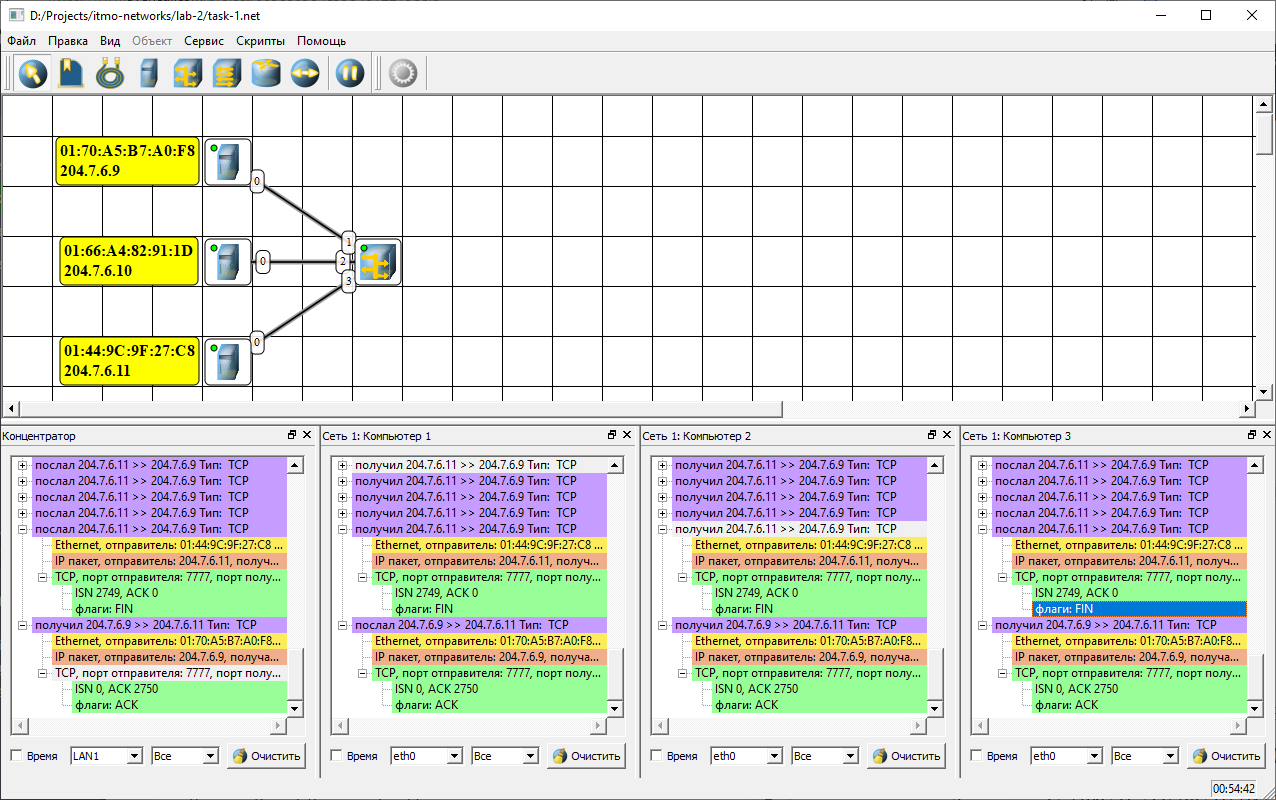
\includegraphics[width=1\linewidth]{res/task-1.png}
    \caption{Этап 1: Схема сети 1 с $N_1=3$ компьютеров соединенных концентратором}
    \label{fig:task-1}
\end{figure}

\Subsection{Этап 2}

Процесс настройки сети для этого этапа аналогичен процессу настройки для  предыдущего этапа. 

Теперь при общении в сети пакеты получают только устройства участвующие в коммуникации: коммутатор и компьютеры 1 и 3, компьютер 2 не получает не предназначенных ему пакетов, но лишь в том случае, если в коммутаторе есть настроенная (в том числе динамически) таблица маршрутизации.

\begin{figure}[H]
    \centering
    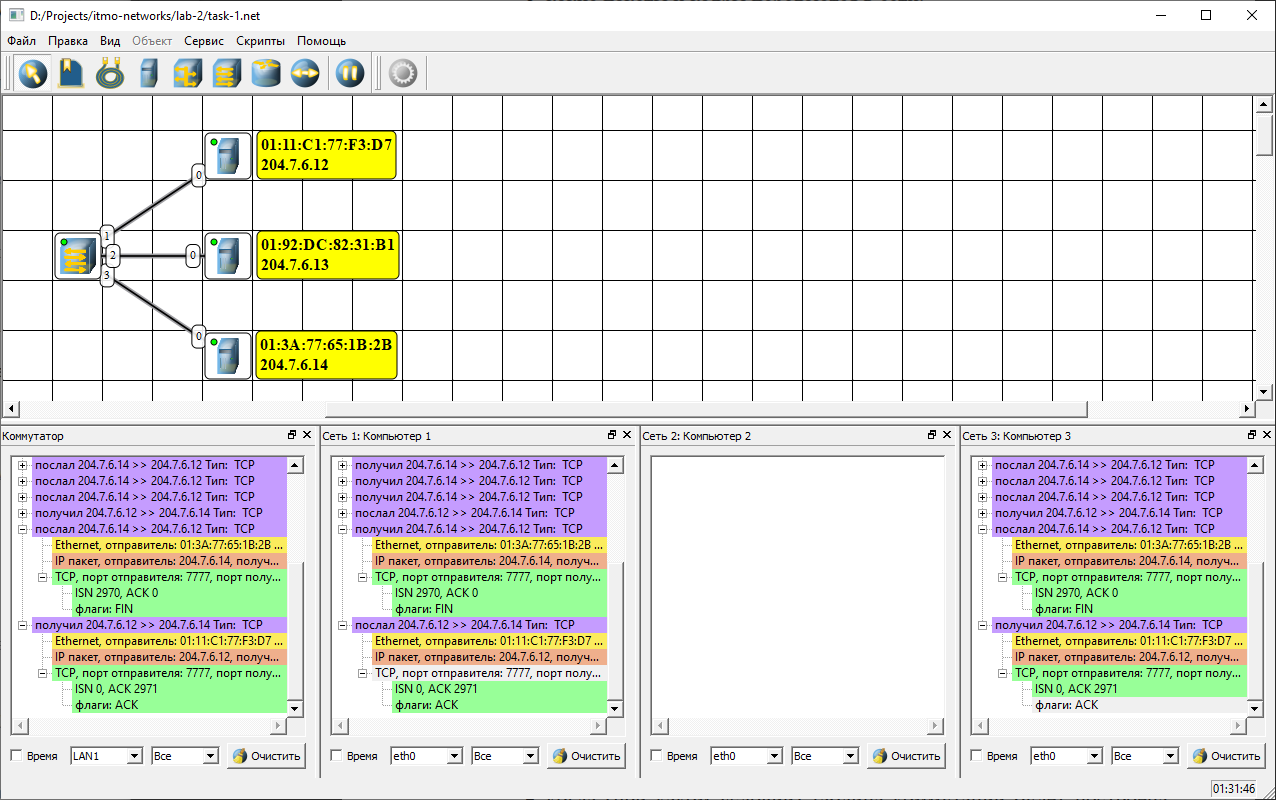
\includegraphics[width=1\linewidth]{res/task-2.png}
    \caption{Этап 2: Схема сети 2 с $N_2=2$ компьютеров соединенных коммутатором (представлено 3 компьютера для демонстрации работы)}
    \label{fig:task-2}
\end{figure}

\Subsection{Этап 3}

Процесс настройки сети для этого этапа аналогичен настройке для предыдущих этапов. Коммутатор третьей сети подключается к коммутатору второй сети, т.к. у них обоих есть свободные LAN-порты (из 4 заявленных).

При передаче пакетов, в случае если отправитель не знает адреса получателя, отправитель посылает запрос на поиск нужного адреса через коммутатор/концентратор и получив ответ, посылает полезные данные, а отправитель сохраняет информацию о получателе в своет ARP-таблице. Таким образом сеть автоматически конфигурируется без дополнительных настроек

\begin{figure}[H]
    \centering
    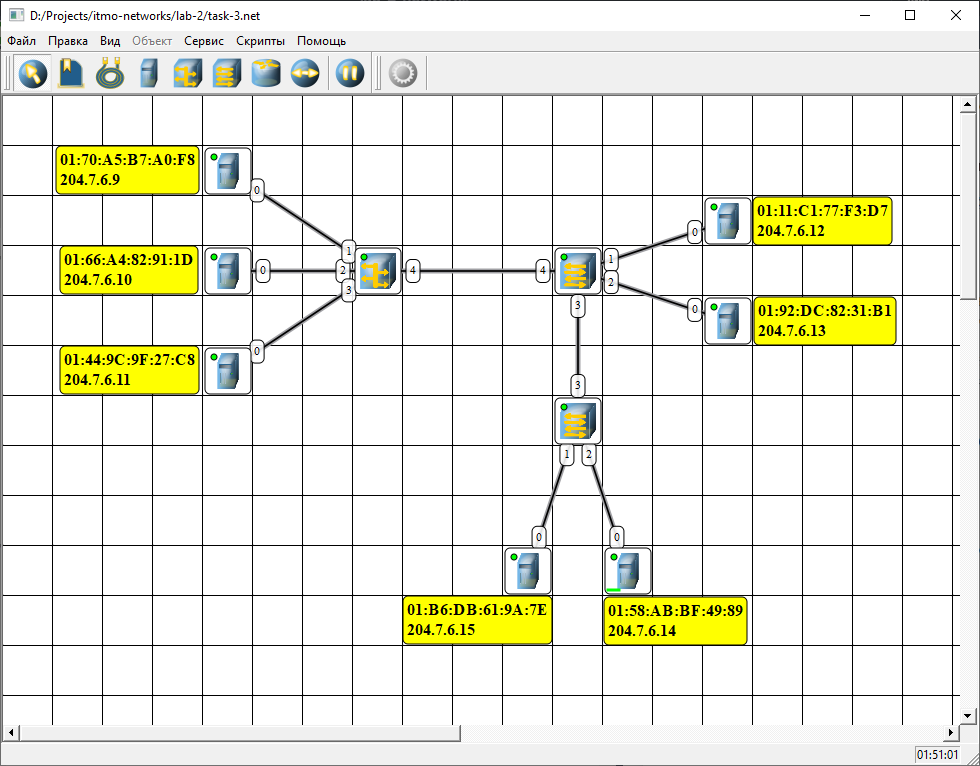
\includegraphics[width=1\linewidth]{res/task-3.png}
    \caption{Этап 3: Схема сети 3 с $N_3=2$ компьютеров соединенных коммутатором}
    \label{fig:task-3}
\end{figure}

% \begin{figure}[H] % 'H' -- вставить тут же (подключен модуль), обычный вариант: 'htpb'
%     \centering
%     % { граница для иллюстрации
%     % \setlength{\fboxsep}{0pt}% убрать отсутп от границы
%     % \setlength{\fboxrule}{1pt}%
%     % \fbox{%
%             \includegraphics[width=\textwidth]{res/UML-class-diagram.png}
%     % }} % ограничение области действия параметров
%     \caption{Caption}
%     \label{fig:enter-label}
% \end{figure}

% Выполнение задания...

\Section{Вывод}

В результате выполнения работы были построены сегменты локальные сети 1, 2, 3 которые позже были объединены в многосегментную локальную сеть. В первом этапе работы была построена сеть с использованием концентратора, во втором этапе сеть с использованием коммутатора, в третьем этапе сети 1 и 2 были объедены в одну сеть и к ним подключена 3 сеть созданная с помощью коммутатора. При этом никаких настроек кроме указания IPv4-адресов устройств не потребовалось, каждый узел сети способен узнать адрес получателя в сети.

%<<<<<<<<<<<<<<<<<<<<<< КОД РАБОТЫ <<<<<<<<<<<<<<<<<<<<<<<<


\end{document}
%<<<<<<<<<<<<<<<< ,,,,,,,,,,,,,,,,,,,,,,, <<<<<<<<<<<<<<<<<
%<<<<<<<<<<<<<<<<<<< СОДЕРЖИМОЕ ОТЧЕТА <<<<<<<<<<<<<<<<<<<<
